%! Author = ryanb
%! Date = 10/31/2025

% Preamble
\documentclass{amsart}

% Packages
\usepackage{amsmath}
\usepackage{amsrefs}
\usepackage{amsthm}

\usepackage{lipsum}
\usepackage{tikz} % delete when finished
\usepackage{float}

\usepackage{hyperref}

\usetikzlibrary{backgrounds}

\theoremstyle{definition}
\newtheorem{definition}{Definition}[section]

\theoremstyle{plain}
\newtheorem{theorem}{Theorem}[section]


% Document
\begin{document}

    \title{Our Title}
    \author{Ryan Bruno}
    \author{Lucas Johnson}
    \author{Nathan LaCrosse}
    \author{Nick Proctor}
    \date{\today}

    \begin{abstract}
        \lipsum[1]
    \end{abstract}

    \maketitle

    \tableofcontents % uncomment if needed

    \section{Introduction to Planar Graphs}\label{sec:intro}

    \begin{definition}
        A graph $G$ is called a \emph{planar graph} if $G$ can be drawn in the plane without any two of its edges crossing~\cite{ourBook}.
        If $G$ is already drawn in the plane without crossings, then $G$ is a \emph{plane graph}.
    \end{definition}
    Importantly, any graph isometric to a plane graph is therefore planar.
    \begin{center}
        \begin{figure}[H]
            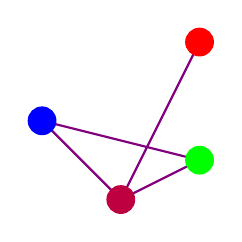
\begin{tikzpicture}[scale=0.5]
                \draw[violet, thick] (0,2) -- (2,0);
                \draw[violet, thick] (2,0) -- (4,1);
                \draw[violet, thick] (4,1) -- (0,2);
                \draw[violet, thick] (2,0) -- (4,4);

                \filldraw [blue] (0, 2) circle (10pt);
                \filldraw [purple] (2, 0) circle (10pt);
                \filldraw [green] (4, 1) circle (10pt);
                \filldraw [red] (4, 4) circle (10pt);
            \end{tikzpicture}
            \hspace{1in}
            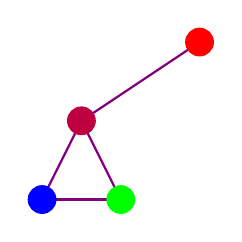
\begin{tikzpicture}[scale=0.5]
                \draw[violet, thick] (0,0) -- (2,0);
                \draw[violet, thick] (2,0) -- (1,2);
                \draw[violet, thick] (1,2) -- (0,0);
                \draw[violet, thick] (1,2) -- (4,4);

                \filldraw [blue] (0, 0) circle (10pt);
                \filldraw [purple] (1, 2) circle (10pt);
                \filldraw [green] (2, 0) circle (10pt);
                \filldraw [red] (4, 4) circle (10pt);
            \end{tikzpicture}\caption{The graph on the left is planar since it is isomorphic to the plane graph on the right.}\label{fig:isomorphicPlanar}
        \end{figure}
    \end{center}
    From here on, when referring to planar graphs, we will be considering the plane graph that the graph is isomorphic to.
    Often, when working with planar graphs, one is concerned with whether or not a given graph is planar.
    This question appears often in contexts where there are connections on a $2D$ gid and intersections are impossible.

    In order to solve this, we must discuss what properties define a planar graph.
    One important theorem is the Euler Identity.

    \begin{theorem}[The Euler Identity~\cite{ourBook}]
        For every connected plane graph of order $n$, size $m$ and having $r$ regions,
        \[n-m+r=2.\]
    \end{theorem}

    In order to be able to understand this theorem, let us first discuss the regions of a graph.
    A \emph{region} is an area bounded by the edges and vertices of a graph $G$.
    Additionally, there is an external region which is unbounded.
    \begin{figure}[H]
        \centering
        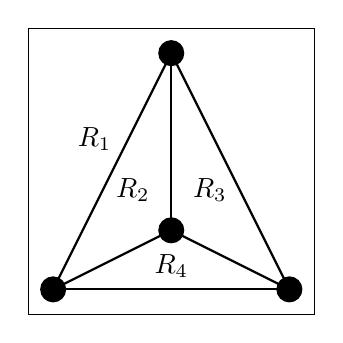
\begin{tikzpicture}[scale=0.75, show background rectangle]
            \draw[black, thick] (0,0) -- (2,4);
            \draw[black, thick] (0,0) -- (2,1);
            \draw[black, thick] (0,0) -- (4,0);

            \draw[black, thick] (2,1) -- (2,4);
            \draw[black, thick] (2,1) -- (4,0);

            \draw[black, thick] (2,4) -- (4,0);

            \filldraw [black] (2, 1) circle (6pt);
            \filldraw [black] (4, 0) circle (6pt);
            \filldraw [black] (0, 0) circle (6pt);
            \filldraw [black] (2, 4) circle (6pt);

            \node[above=0.75in, right=0.075in] at (0,0) {$R_1$};
            \node[above=0.2in, left=0.06in] at (2,1) {$R_2$};
            \node[above=0.2in, right=0.06in] at (2,1) {$R_3$};
            \node at (2,0.4) {$R_4$};
        \end{tikzpicture}
        \caption{A planar graph with its regions denoted.}
        \label{fig:regions}
    \end{figure}

    With this in mind, let us prove Euler's Identity.
    \begin{proof} Proceed by induction.
        \begin{enumerate}
            \item \emph{Base Case:} Consider the graph $K_1$, of order $1$, size $0$ and containing one region.
                Since there are no possible edges that could cross, the induction holds.
            \item \emph{Inductive Hypothesis:} If we assume that the hypothesis holds for a graph of order $n$, size $m$ and $r$ regions, then we will show it holds for a graph of order $n$, size $m=1$ and
        \end{enumerate}
    \end{proof}

    ??

    The Euler Identity is a powerful tool in characterizing planar graphs.
    However, it is difficult to determine the amount of regions in an arbitrary graph.
    Luckily, the Euler Identity leads to a result that no longer requires a region count.
    Since each edge is on the boundary of at most two regions in a graph $G$, we can use the Euler Identity to get a result in terms of the order and size of $G$.

    If $G$ is a planar graph of order $n\geq 3$ and size $m$, then
    \[m\leq 3n-6.\]
    Equivalently, if $G$ is of order $n\geq 5$ and size $m$ such that
    \[m>3n-6,\]
    then $G$ is nonplanar.

    These results lead to two important nonplanar graphs that leas to a universal planarity criterion.
    Namely, both $K_5$ and $K_{3,3}$ are nonplanar.
    $K_5$ is of order $5$ and size $20$, and since $20>15-6$, it is therefore nonplanar by our newest result.
    $K_{3,3}$ is of order $6$ and size $9$, so we can't say anything using the size formulas.
    Instead, the Euler identity requires that $6-9+r=2$.
    Therefore, $K_{3,3}$ must have $5$ regions to be nonplanar.
    However, since bipartite graphs have no odd cycles, each region of the graph requires at least four edges on the boundary (boundaries are cycles).
    Since each edge in $K_{3,3}$ is on a cycle, it is on the boundary of two regions -- so each edge gets counted twice when constructing these regions.
    Therefore, the minimum size of $K_{3,3}$ must be $\frac{5\times 4}{2}=10$.
    However, since $K_{3,3}$ is of size $9$, this is impossible -- sp $K_{3,3}$ must be nonplanar.

    \begin{figure}[H]
        \centering

        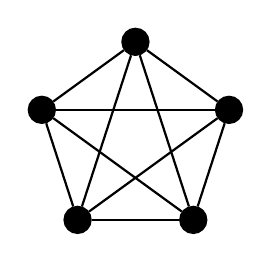
\begin{tikzpicture}[
            vertex/.style = {
                circle,
                draw,
                thick,
                fill=black,
                minimum size=1mm,
                font=\sffamily
            }
        ]
            \def\numVertices{5}
            \def\radius{1.25}
            \foreach \i in {1,...,\numVertices} {
                \node[vertex] (v\i) at ({90 - (\i - 1) * (360/\numVertices)}:\radius) {};
            }
            \draw[thick, color=black] (v1) -- (v2);
            \draw[thick, color=black] (v1) -- (v3);
            \draw[thick, color=black] (v1) -- (v4);
            \draw[thick, color=black] (v1) -- (v5);

            \draw[thick, color=black] (v2) -- (v3);
            \draw[thick, color=black] (v2) -- (v4);
            \draw[thick, color=black] (v2) -- (v5);

            \draw[thick, color=black] (v3) -- (v4);
            \draw[thick, color=black] (v3) -- (v5);

            \draw[thick, color=black] (v4) -- (v5);

        \end{tikzpicture}\hspace{1in}
        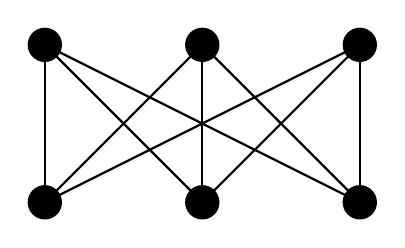
\begin{tikzpicture}
            \draw[black, thick] (0,0) -- (0,2);
            \draw[black, thick] (0,0) -- (2,2);
            \draw[black, thick] (0,0) -- (4,2);

            \draw[black, thick] (2,0) -- (0,2);
            \draw[black, thick] (2,0) -- (2,2);
            \draw[black, thick] (2,0) -- (4,2);

            \draw[black, thick] (4,0) -- (0,2);
            \draw[black, thick] (4,0) -- (2,2);
            \draw[black, thick] (4,0) -- (4,2);

            \filldraw [black] (0, 0) circle (6pt);
            \filldraw [black] (0, 2) circle (6pt);
            \filldraw [black] (2, 0) circle (6pt);
            \filldraw [black] (2, 2) circle (6pt);
            \filldraw [black] (4, 0) circle (6pt);
            \filldraw [black] (4, 2) circle (6pt);
        \end{tikzpicture}

        \caption{$K_5$ (left) and $K_{3,3}$ (right), two nonplanar graphs.}
        \label{fig:k_5k_33}
    \end{figure}

    Put simply, the idea behind the universal criterion for planarity is the following: can we show that a given graph has the same kind of geometry as $k_5$ or $K_{3,3}$?
    Furthermore, we only have to show that a part of a graph has this geometry -- as there only needs to be one instance of line crossing to have a nonplanar graph.
    To do this, we use the power of edge contractions.

    \section{title}
    f

    \section{title}
    f

    \section{Applications of Planar Graphs}\label{sec:applications}
    When discussing applications of planar graphs, the first thing that might come to mind would resie in the field of civil engineering.
    Roads, bridges, and traffic flows are all operations of which general graph theory is very apparent.
    Intersections and roads can be thought of as graphs with edges and vertices.
    The crossing of edges, or in this case roads, requires a decision to be made whether to implement a new intersection or a bridge overpass.
    While both options are viable, bridges cost significantly more in every aspect.

    So how do planar graphs make traffic planning optimal?
    Since planar graphs have no intersecting or crossing edges, civil engineers can optimize the placement of intersections and roads to understand if there exists somewhere a bridge is absolutely necessary or an opportunity to save time and money by avoiding bridge construction outright.

    What other applications might exist?
    From a network engineer perspective, graphs can represent entire networks.
    Data being transferred by ethernet consists of eight electrical pulses through copper wire which are subject to electrical interference.
    If too many cables cross, packet loss may occur, leading to the user experience slowing down.
    Similarly, Electrical Engineers become subject to the same issue or interference.
    When designing a single layered Printed Circuit board (PCB), engineers must keep the layout planar, as adding in Vias leads to increased complexity, cost, and resistance on the board.

    \newpage

    % bibliography stuff goes here
    \begin{bibdiv} % "produces the chapter or section heading for the bibliography" (the thing that says 'REFERENCES')
        \begin{biblist} % contains the reference list

            % may add more data to this
            \bib{ourBook}{book}{
                title={Graphs and Digraphs},
                author={Gary Chartrand},
                author={Linda Lesniak},
                author={Ping Zhang},
                date={2016},
                publisher={CRC Press},
                address={Boca Raton}
            }

            \bib{grassl}{webpage}{
                title={More Discrete Mathematics via Graph Theory},
                author={Richard Grassl},
                author={Oscar Levin},
                date={2018},
                url={https://discrete.openmathbooks.org/more/mdm/mdm.html}
                accessdate={November 17, 2025}
            }

        \end{biblist}
    \end{bibdiv}

\end{document}
